\begin{figure}[H]
    \centering
    \scalebox{0.7}{
    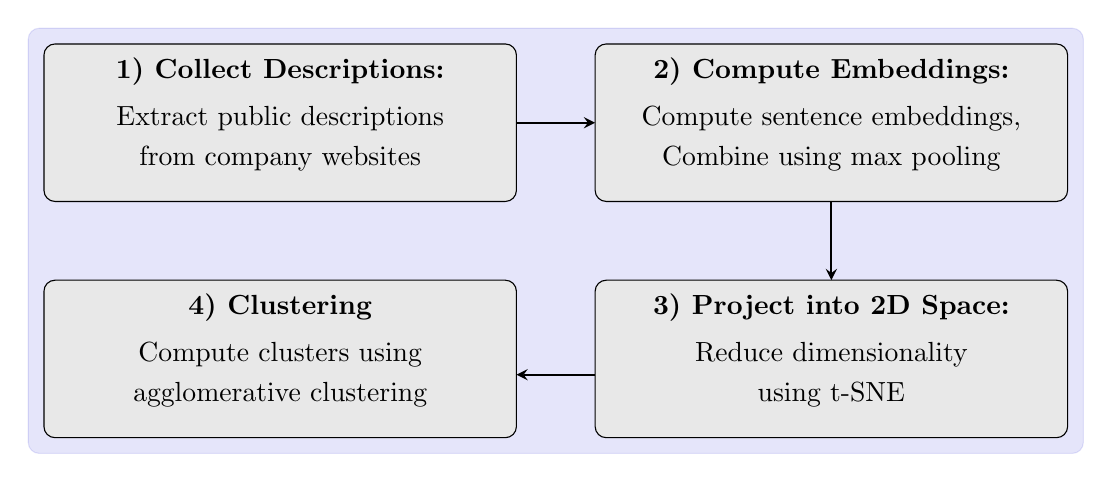
\begin{tikzpicture}
        \definecolor{lightgrey}{RGB}{232,232,232}
        \definecolor{darkblue}{RGB}{0,0,204}
        
        \draw[rounded corners, darkblue, fill=darkblue, opacity=0.1] (-9.2, 0) rectangle (4.2, 5.4);    
         
         \draw[rounded corners, fill=lightgrey] (-9, 3.2) rectangle (-3, 5.2);
         \node[font=\bfseries] at (-6, 4.85) {1) Collect Descriptions:};
         \node at (-6, 4.25) {Extract public descriptions};
         \node at (-6, 3.75) {from company websites};
         \draw[thick, -stealth] (-3, 4.2) -- (-2, 4.2);
         
         \draw[rounded corners, fill=lightgrey] (-2, 3.2) rectangle (4, 5.2);
         \node[font=\bfseries] at (1, 4.85) {2) Compute Embeddings:};
         \node at (1, 4.25) {Compute sentence embeddings,};
         \node at (1, 3.75) {Combine using max pooling};
         \draw[thick, -stealth] (1, 3.2) -- (1, 2.2);
          
          \draw[rounded corners, fill=lightgrey] (-2, 0.2) rectangle (4, 2.2);
          \node[font=\bfseries] at (1, 1.85) {3) Project into 2D Space:};
          \node at (1, 1.25) {Reduce dimensionality};
          \node at (1, 0.75) {using t-SNE};
          \draw[thick, -stealth] (-2, 1) -- (-3, 1);
       
          \draw[rounded corners, fill=lightgrey] (-9, 0.2) rectangle (-3, 2.2);
          \node[font=\bfseries] at (-6, 1.85) {4) Clustering};
          \node at (-6, 1.25) {Compute clusters using};
          \node at (-6, 0.75) {agglomerative clustering};
         
    \end{tikzpicture}}
    \caption{Overview of our clustering pipeline.}
    \label{fig:pipeline}
\end{figure}
